\documentclass{article}
\usepackage{imakeidx}
\usepackage{graphicx}
\usepackage{wrapfig}
\usepackage{mathtools}
\graphicspath{{images/}}
\usepackage{geometry}
\geometry{a4paper,
total={170mm, 257mm},
left = 30mm,
right = 30mm,
bottom = 30mm,
top = 30mm
}

\usepackage{multicol}
\title{C/C++\linebreak Revision Notes}
\author{James Brown}
\makeindex
\begin{document}
	\pagenumbering{gobble}
	\maketitle
	\newpage
	\tableofcontents
	\newpage
	\pagenumbering{arabic}

	\section{Introduction}
	These are notes I have written in preparation of the 2017 C/C++ exam. This year the module was run by Hayo Thielecke (H.Thielecke@cs.bham.ac.uk). This module focuses on the features of C and C++ that are important in Computer Science in general. It is not a rerun of the first year Software Workshop module.
	\linebreak \linebreak
	
	\section{Pointers and Memory Management}
	\subsection{Pointers}	
	Pointers are a fundamental feature of C which have not been encountered in programming languages we have used to this point, and they are used everywhere in C. What is the meaning of \texttt{x = x + 1;}? It does not mean $2 = 2 + 1$. The \texttt{x} on the left side of the \texttt{=} refers to the address (L-value) \texttt{x}. The \texttt{x} on the right side of the \texttt{=} refers to the contents (R-value) of \texttt{x}. Here, the L-value is a \textbf{pointer}\index{pointer}
	
	\par 
	The view of memory in C is of a graph, as we would like to abstract away from actual hardware addresses. Nodes in the graph are chunks of memory (often this is a struct), and edges between nodes are pointers. Due to this, box-and-arrow diagrams are very useful in representing the state of memory.
	
	\begin{figure}[ht]
		\begin{minipage}[t]{0.45\textwidth}
			\centering
			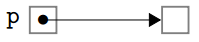
\includegraphics[width=0.45\textwidth]{box_arrow_diagram}
			\caption{A box-and-arrow diagram}
			\label{fig:bow arrow diagram}
		\end{minipage}
		\hfill
		\begin{minipage}[t]{0.45\textwidth}
			\centering
			
\includegraphics[width=0.45\textwidth]{box_arrow_diagram_memory}
			\caption{The hardware level of a box-and-arrow diagram}
			\label{fig:box arrow diagram memory}
		\end{minipage}
	\end{figure}	
		
	\subsubsection{The * and \& Operators}
	In C, * is also a unary operator. It is also used for binary multiplication, but the two have nothing to do with each other. If \texttt{P} is an expression denoting a pointer, then \texttt{*P} is the result of derefencing the pointer (that is getting the value of the thing it points to in memory). If \texttt{T} is a type, then \texttt{T *p;} declares \texttt{p} to be of type 'pointer to \texttt{T}'. If \texttt{T} is a type, then \texttt{T*} is the type of pointers to something of type \texttt{T} - this is used in casting. Important to note is that the \texttt{*} does not stick to everything in a declaration. For example, \texttt{int *p, n;} is like:
	
	\begin{verbatim}
	int *p;
	int n;
	\end{verbatim}
	
	and not
	
	\begin{verbatim}
	int *p;
	int *n;
	\end{verbatim}
	
	Care should be taken when defining pointers in this fashion.	
	
	\par 
	If a variable appears on the right-hand side of an \texttt{=}, its R-value is taken. If we want to get the address of a variable rather than its contents, we use the \texttt{\&} operator - \texttt{\&x} for example.
	
	\par 
	In C, two pointers are \texttt{==} if they refer to the same address in memory. Pointer equality is different from structural equality that is built into other languages. \texttt{p = q}  makes \texttt{p == q}. \texttt{*p = *q} does not make \texttt{p == q}.
	
	\subsubsection{The Null Pointer}
	There is a special pointer value, called the \textbf{null} pointer. In C, it is called the \texttt{NULL} pointer and in C++ it is called the \texttt{nullptr}. The null pointer, unsuprisingly, does not point to anything. Derefencing \texttt{NULL} will give an undefined behaviour (usually this will be a crash). In C, we have an idiom to test whether a point \texttt{p} is equal ot the null pointer:
	\begin{verbatim}
	if(p) ...
	\end{verbatim}
	
	It is important to note that pointers are not always initialised to null. 
	
	\subsection{Memory Management with \texttt{malloc} and \texttt{free}}
	In C, \texttt{stdlib.h}\index{stdlib.h} provides the functions \texttt{malloc}\index{malloc} and \texttt{free}\index{free}. The part of memory managed by \texttt{malloc} is called the \textbf{heap}\index{heap}. \texttt{malloc} allows us to borrow some memory from the memory manager, and \texttt{free} allows us to give back the memory that we have borrowed. We must promise to not use the memory that we have freed again, although the memory manager cannot force us not to do this. Regardless we still should not touch freed memory has it can lead to undefinied behaviour. Also important to note is that the call to \texttt{free} changes the ownership of the memory, not any of the pointer which pointed to that memory. The \texttt{free} operator is very important, as our program will leak memory otherwise. Luckily, we have tools such as Valgrind to help us analyse our code and test for memory errors and leaks.
	
	\par 
	\texttt{malloc} and \texttt{free} are not part of the C language itself, only its standard library. Due to this, we could implement our own memory allocator in C if we so wish. The allocator would request some memory from the OS (this would be done via \texttt{sbrk} in Unix). The available memory would be divided into chunks that are linked together in a 'free list'. A call to \texttt{malloc} will then detach a chunk from the free list and return a pointer to it. A call to \texttt{free} takes the pointer to the chunk and links it back into the free list. This is not massively efficient and may also result in memory fragmentation, but the fact we can do it is still impressive.
	
	\par 
	What happens once \texttt{free} is called upon some memory? Various things: the same piece of memory may be used again in a later \texttt{malloc}, or the memory manager might write its own data structures into the memory (e.g. the free list). Rather than trying to guess exactly what happens, we simply call it undefined behaviour. C, unlike other languages, will not prevent you from doing bad things with freed memory. 
	
	Using \texttt{malloc} and \texttt{free} we could write a piece of example code like such:
	\begin{verbatim}
	int *p1, **p2;
	p1 = malloc(sizeof(int));
	*p1 = 7;
	p2 = malloc(sizeof(int*));
	*p2 = p1;
	free(p1);
	\end{verbatim}
	
	If we add the line \texttt{**p2 = 11;} as the last line of this piece of code, we would be adding an example of use after free, which we should absolutely avoid doing!
	
	\subsubsection{The \texttt{sizeof} operator}
	For using \texttt{malloc}, we need to tell the function how many bytes to allocate. Usually, we are allocating enough memory to hold a specific type, but sizes of types are implementation dependent. The compiler will tell us how big it makes each type, and this can be found by using \texttt{sizeof(T)}. Very commonly we will write a piece of code as follows:
	
	\begin{verbatim}
	T *p = malloc(sizeof(T));
	\end{verbatim}
	
	\subsubsection{Crashes vs Memory Errors}
	In C, crashes and memory errors are not the same thing. Crashes usually have many names, such as core dumps\index{core dump} or segmentation faults\index{segmentation fault}\index{segfault}. Crashes are errors which have been detected by the hardware or the OS. In C, a memory error \textit{may} lead to a segfault, but it is not guaranteed that it will. A write error which does not lead to a segfault may instead lead to corrupted memory - this could be even worse! A C program with a memory error is always wrong. A memory leak is not the same as a memory error, and not always a bad situation. A memory leak may lead to a crash though when the program eventually runs out of memory.
	
	\section{Structures in C}
	A structure (or \texttt{struct}) is much like a Java class that contains only data and no methods.	
	
	\section{Typed Trees in C}

	\section{From C and Java to C++}
	
	\section{Templates in C++}
		
	\newpage
	\listoffigures
	\printindex
\end{document}